KD-Tree is a space partitioning structure which can be used to organise data points in k dimensional space. We have fixed our dimensions of data points  to 2-dimensions and their values are stored in 1-dimension. In our implementation KD-Tree is a binary tree with every node having data points partitioned in 2-dimensional space.\\\\\

\subsubsection{Definitions}

\begin{figure}[htp]
    \centering
    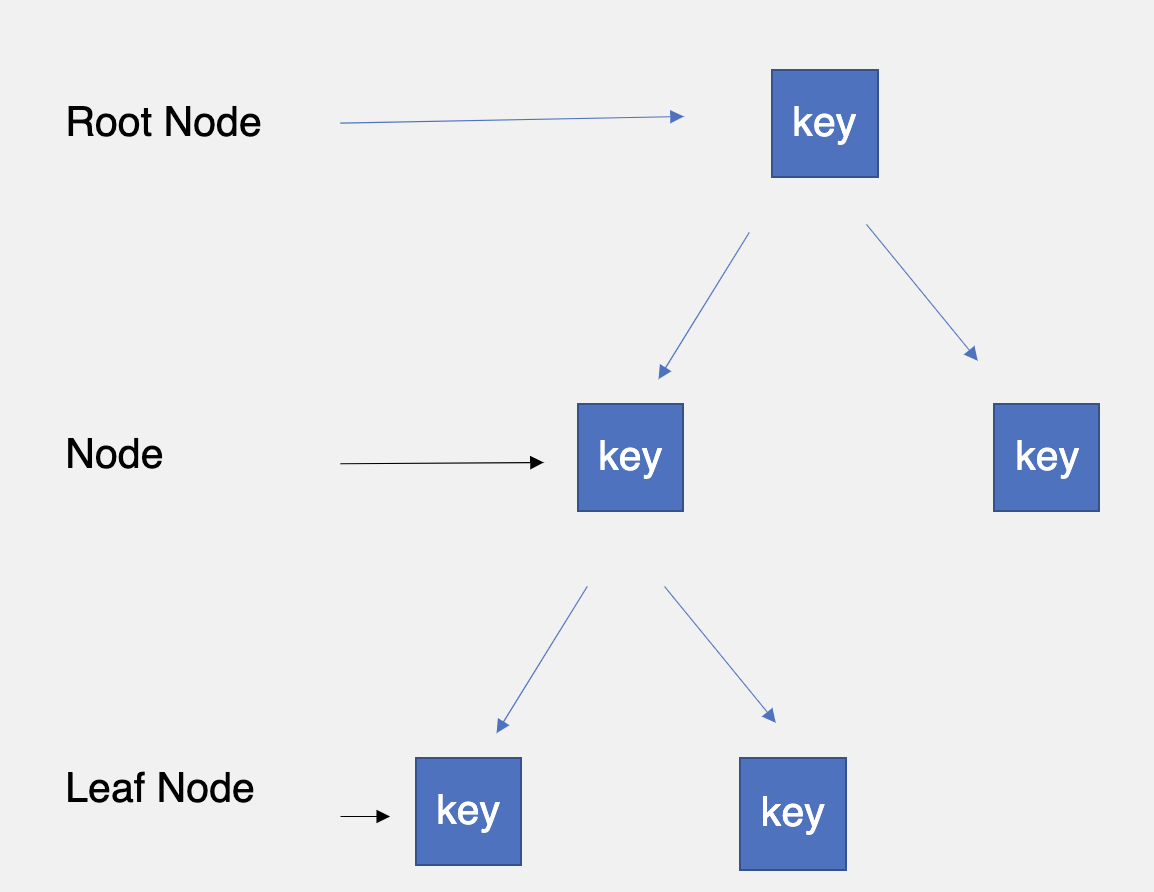
\includegraphics[width=0.6\textwidth]{graphs/KD-Tree.png}
    \caption{KD-Tree}
    \label{fig:KD-Tree}
\end{figure}

\begin{enumerate}
    \item\textbf{{Node}}: Node of a KD-Tree is essentially a 2-dimensional data point. It can be k-dimensional for KD-Tree.
    \item\textbf{{Root Node}}: Root Node is the Node with no parents and has other nodes/leaves as children. Each node can have two child nodes since it is a binary tree. 
    \item\textbf{{Leaf Node}}: Leaves of a tree are the nodes which do not have any child nodes.
    \item\textbf{{Dimensions}}: Every KD-Tree can be structured in such a way that the data points are divided into k-dimensions. Each node is recursively cut into as many dimensions as is mentioned in the dimensions. In our case the data points are 2-dimensional and hence the space is divided in 2-dimensions alternatively until a leaf is reached.\\
\end{enumerate}
    
\begin{algorithm}[H]
    \SetAlgoLined
    \SetKwInOut{Input}{Input}
    \SetKwInOut{Output}{Output}
    \Input{Point list; trainset=[$(x,y);x \in \mathbb{R}^{2};y \in \mathbb{R}$], dimension = 2, $int$ split axis; 0 or 1}
    \Output{KD-Tree}
    \For{$i\gets0$ \KwTo $len(Point list)$}{
    \texttt{$int$ split axis := split axis mod $dim$} // Select the split axis based on depth\\
    \texttt{Sort point list and choose median}\\
    \texttt{Create node at median}\\
    \texttt{node.leftChild := kdtree(points in pointList before median, split axis+1); //SubTree Creation \\ 
    node.rightChild := kdtree(points in pointList after median, split axis+1);}
     \caption{Training Algorithm for KD-Tree}
     \label{Training_KD-Tree}
     }
\end{algorithm}

For constructing the KD-Tree we have following consttraints:


\begin{enumerate}
    \item {As one moves down the tree, one cycles through the axes used to select the splitting planes. For example, in a 2-dimensional plane we split the data on x-axis at the root and then split it on y-axis for it's children. We then split the grandchildren on x-axis again and so on.}
    \item {Points are inserted by selecting the median of the points being put into the subtree, with respect to their coordinates in the axis being used to create the splitting plane. This ensures that the tree is balanced. A balanced tree is the one in which leaf node is approximately the same distance from the root.}\\
\end{enumerate}    
    
In the algorithm above, we first sort all the values obtained in the Point list. We initialise the first split axis to 0 and then toggle between 0 and 1 as we increase the depth. Once the data points are sorted, their median is chosen. For example if we have points sorted as [[3,4],[5,6],[7,8]], we will take the median as [5,6] and assign [3,4] to the left and [7,8] to the right. The reason node.leftChild = [1,2] is because 1 < 5 and node.rightChild = [7,8] is because 7 > 5 i.e., we compare the x-axis of the points to the root when we create the subsequent nodes. This process is then carried out recursively and subtrees are created on the left and right until all the points are added to the tree from the Point list.

\subsubsection{Construction time of 2-dimensional kd-tree:}

The most expensive part of the construction of KD-Tree is sorting the points on both the axis. Instead of working with more complex algorithm to find the median we first presorted the values on x-axis and then on y-axis. Hence the time complexity is $O( n log n)$. Since KD-Tree is A binary tree, and every leaf and internal node uses O(1) storage, the total storage is $O(n)$.


\subsubsection{Introduction to Range Searching}

\begin{figure}[htp]
    \centering
    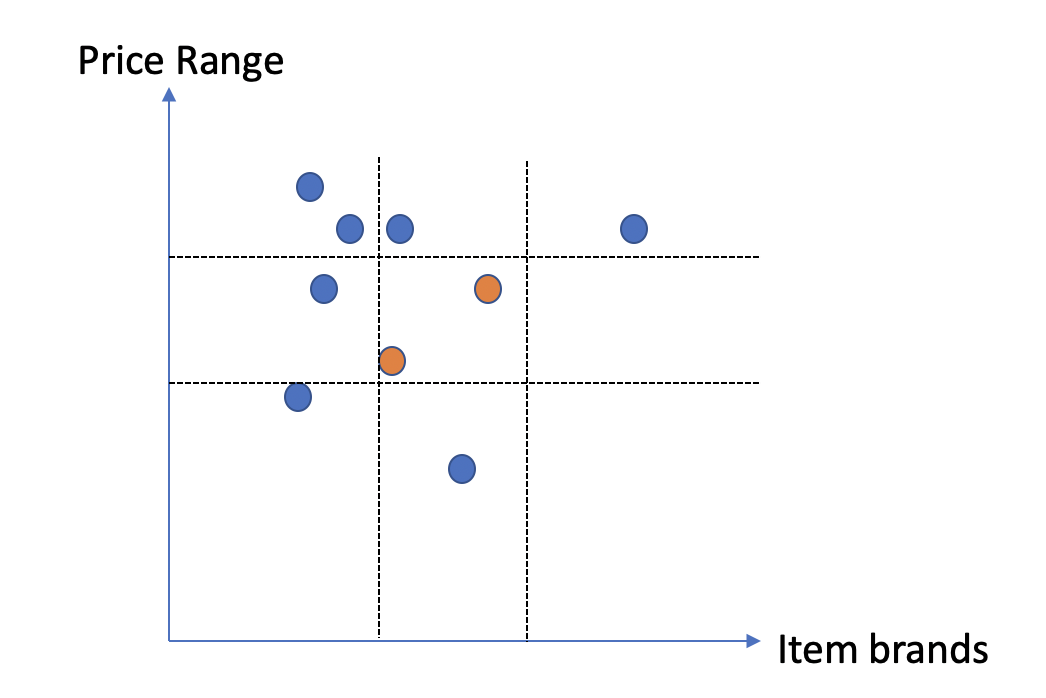
\includegraphics[width=0.6\textwidth]{graphs/Range_Query_Intro.png}
    \caption{KD-Tree Range Query}
    \label{fig:KD_ee_Range_Query_Intro}
\end{figure}

Range searching is basically to search data which lie within a specified range. For example if you have a database where you store data of a number of items and their price ranges. You want to search items from a specific brand and within a specific price range. You can search for this data by specifying these parameters. In our model we can pass the lower bound and upper bound of a rectangle and all the points that lie within those bounds are retrieved in the 2-dimensional plane.


\begin{figure}[htp]
    \centering
    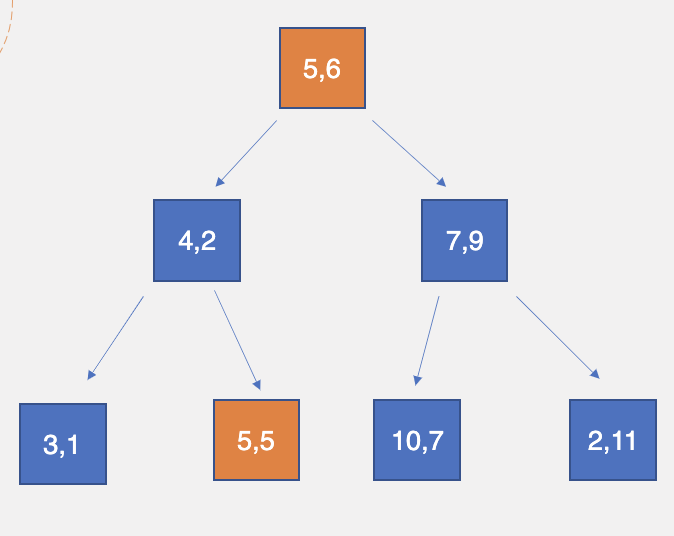
\includegraphics[width=0.6\textwidth]{graphs/Range_Query_Tree.png}
    \caption{KD-Tree for Range Query}
    \label{fig:KD-Tree_for_Range Query}
\end{figure}

\begin{figure}[htp]
    \centering
    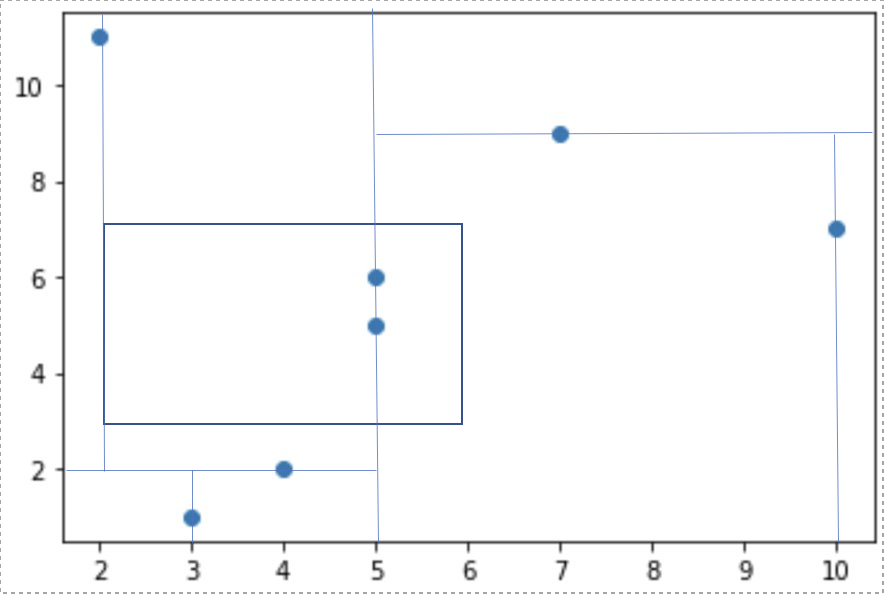
\includegraphics[width=0.6\textwidth]{graphs/Range_Query_plot.png}
    \caption{KD-Tree Range Query Plot on 2-dimentional plane}
    \label{fig:KD_Tree_Range_Query_Plot}
\end{figure}

In our model in range query we first generate lower and upper bound of the rectangle randomly. We then check if the root of the tree lies within the range of the bounds and only then start traversing the tree. For example we have a tree with Point list as 

	$$[(5,6),[4,2],[7,9],[3,1],[5,5],[10,7],[2,11]]$$
	
	and with lower bound = [2,3] and upper bound = [6,7], we will get a tree as is shown in \ref{fig:KD-Tree_for_Range Query}. We can see the points along with the rectangle range plotted in \ref{fig:KD_Tree_Range_Query_Plot}. Points [5,5] and [5,6] are returned in the query since they lie within the rectangle as seen in the plot. First the root point is checked and since the x coordinate and y coordinate both lie within the rectangle bounds i.e., 2 > 5 > 6 and 3 > 6 > 7. It then checks if the x coordinate is lower than or greater than the lower bound x coordinate. Since the value is larger than lower bound x coordinate that is 2 it will then traverse to the left. In the left it has child node as [4,2] however, since the y coordinate doesn't lie in the range of the upper bound this point is not selected. Therefore, it recursively traverses the tree and checks if the point lies within the bound until it reaches a leaf.

\subsubsection{K-nearest neighbour}

K-nearest neighbour as the name suggests is the process to find the k nearest neighbour to the test point that we are looking for. For example in a database if you have coordinates of various famous restaurants stored and you want to query 5 nearest restaurants to your current location then the query should fetch you 5 nearest restaurants depending on your current location on the map. Your current coordinate can be any value and may not be a subset of the data. \\

In our model k-nearest neighbour is calculated based on the euclidean distance of the test data point with respect to the other points. We have also compared the result of our model with standard packages of scipy sklearn to verify the results of the distance calculated and the points returned. Since measuring distance of each point from the test point is computationally very expensive we exploit the tree structure of the KD-Tree to prune the tree and only measure distance with much fewer points and only traverse a subtree if required. \\

\begin{figure}[htp]
    \centering
    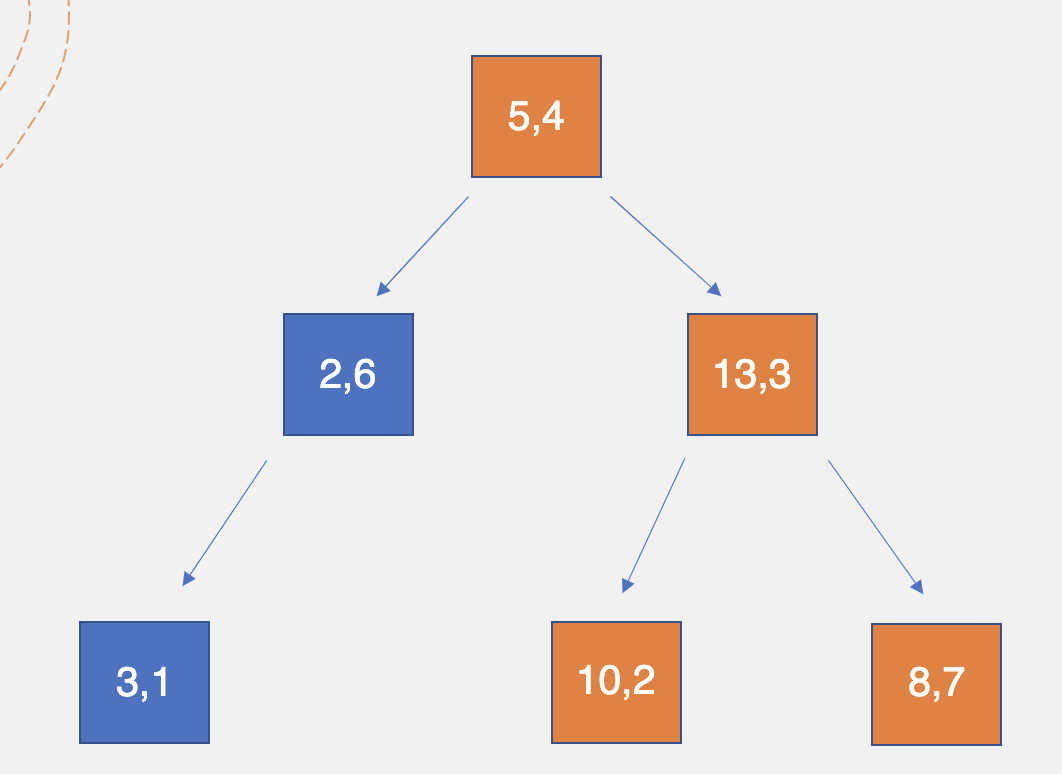
\includegraphics[width=0.6\textwidth]{graphs/KD-Tree_KNN_Tree.png}
    \caption{KD-Tree for KNN Query}
    \label{fig:KD-Tree_for_KNN Query}
\end{figure}

\begin{figure}[htp]
    \centering
    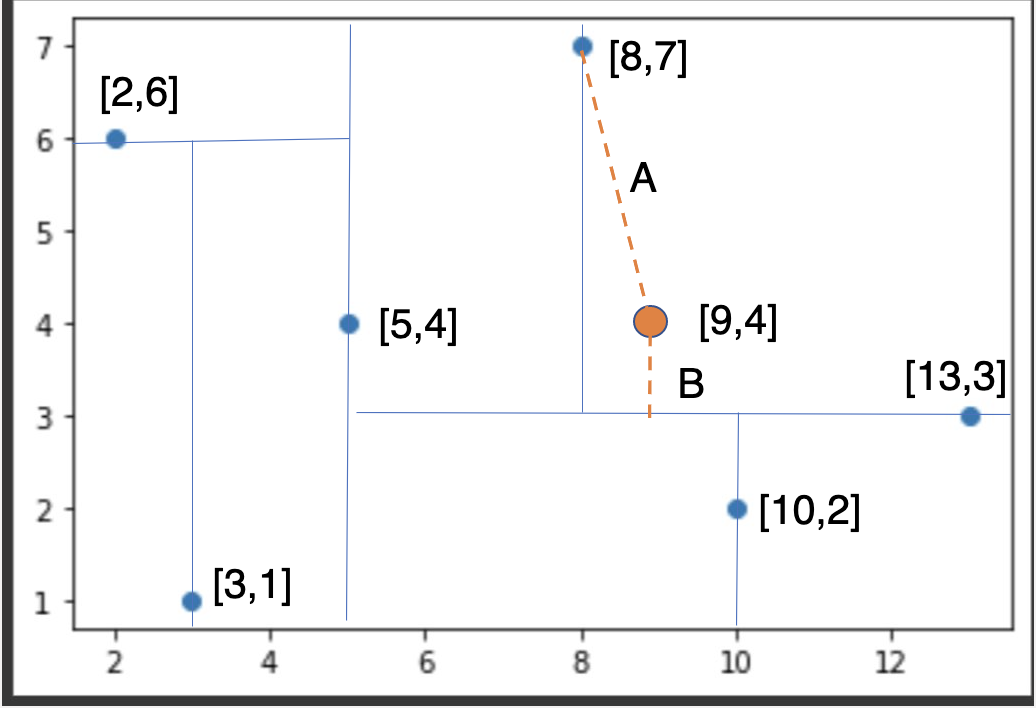
\includegraphics[width=0.6\textwidth]{graphs/KD-Tree_KNN_plot.png}
    \caption{KD-Tree KNN Plot on 2-dimentional plane}
    \label{fig:KD_Tree_KNN_Plot}
\end{figure}


\begin{mscexample}
	For example, we have Point list as $[(5,4),[2,6],[13,3],[8,7],[3,1],[10,2]]$ then we will have a tree structure as shown in \ref{fig:KD-Tree_for_KNN Query} and it's plot on 2-dimensional plane is shown in \ref{fig:KD_Tree_KNN_Plot}. As we can see in \ref{fig:KD_Tree_KNN_Plot} that even though point [8,7] is the leaf we will reach when we traverse the tree to search for point nearest to test point [9,4] it is not infact the nearest point to the test data. In this case if we want to look for 4 nearest neighbour, we first check the square of euclidean distance of [9,4] with the root of the tree i.e., [5,4] which is 16. It then calculates the distance with [2,6] and [13,3] which calculates to 53 and 17 respectively. It then keeps traversing to the right node while calculating distance until it reaches a leaf. After reaching the leaf it then checks the distance with [8,7] with a distance of 10 which is infact smaller than the previous shortest distance of 16 with the root. It adds these points to the list. It then makes a decision weather to go left from [13,3] based on the distance of the test point with leaf [8,7] i.e., A and the perpendicular distance with point [13,3] which is B. Since distance A > B as can be seen in the figure \ref{fig:KD_Tree_KNN_Plot} there is a chance that there could a point in the subtree with a distance smaller than the previous points. In this case it will then check the distance with point [10,2] and the distance is the shortest(best distance) so far of 5. 
\end{mscexample}

